\section{Additional Tables} \label{sec:appxa}

\subsection{Full set of Treatment Effects for Median Housing Price}

The full set of treatment effects in Table \ref{tab:median_sale_amount_full} supports Table \ref{tab:median_sale_amount}, which provides treatment effects for the housing price outcome variable in the main body of the paper. These treatment effects are estimated using a regression discontinuity model explained in Section \ref{sec:empirical}. Additionally, Table \ref{tab:median_sale_amount_winsorized} presents the treatment effects after applying 1\% Winsorization to the data, ensuring robustness against outliers. Furthermore, Table \ref{tab:urban_rural_results} breaks down the treatment effects by urban and rural categories, highlighting the differential impacts on housing prices based on the urbanization level.

\begin{table}[htbp]
    \centering
    \caption{Full set of estimates - Median Housing Price}
    \label{tab:median_sale_amount_full}
    \begin{tabular}{p{3cm}cccc}
        \hline
        \textbf{Year relative to vote} & \textbf{Estimate} & \textbf{Std. error} & \textbf{\textit{p-value}} & \textbf{Confidence interval} \\
        \hline
        $t - 3$  & 5,295   & 7,255  & 0.466  & [-8,926, 19,515] \\
        $t - 2$  & 247     & 6,969  & 0.972  & [-13,412, 13,907] \\
        $t - 1$  & -258    & 7,594  & 0.973  & [-15,141, 14,626] \\
        $t + 1$  & -3,815  & 8,502  & 0.654  & [-20,480, 12,849] \\
        $t + 2$  & -10,829 & 8,840  & 0.221  & [-28,156, 6,497] \\
        $t + 3$  & -14,437 & 7,782  & 0.064  & [-29,691, 817] \\
        $t + 4$  & -21,684 & 7,838  & 0.006  & [-37,047, -6,321] \\
        $t + 5$  & -22,415 & 8,348  & 0.007  & [-38,777, -6,052] \\
        $t + 6$  & -17,539 & 8,465  & 0.038  & [-34,130, -947] \\
        $t + 7$  & -16,001 & 6,918  & 0.021  & [-29,560, -2,442] \\
        $t + 8$  & -21,973 & 9,111  & 0.016  & [-39,830, -4,116] \\
        $t + 9$  & -19,890 & 7,756  & 0.010  & [-35,092, -4,687] \\
        $t + 10$ & -16,042 & 8,915  & 0.072  & [-33,515, 1,432] \\
        \hline
    \end{tabular} 
    \begin{tablenotes}
        \small
        \item \textit{Notes:} Supplements Figure 4 in text. Full set of treatment effect estimates of cutting road tax levies relative to renewing road tax levies from 3 years before the vote to 10 years after the vote. Covariates from Table \ref{tab:variable_means_sd} used in all regressions. Outcome is median house price in constant 2010 U.S. dollars. Unit of observation is the city-year. A treatment effect of -\$21,684 means that four years after the vote, cities that vote to cut road taxes and its associated spending have houses that sell for \$21,684 less than cities that vote to renew road taxes and spending.
    \end{tablenotes}
\end{table}

\begin{table}[htbp]
    \centering
    \caption{Full set of estimates - Median Housing Price (after 1\% Winsorization)}
    \label{tab:median_sale_amount_winsorized}
    \begin{tabular}{p{3cm}cccc}
        \hline
        \textbf{Year relative to vote} & \textbf{Estimate} & \textbf{Std. error} & \textbf{\textit{p-value}} & \textbf{Confidence interval} \\
        \hline
        $t - 3$  & 286     & 6,334  & 0.964  & [-12,128, 12,701] \\
        $t - 2$  & 1,878   & 6,320  & 0.766  & [-10,509, 14,266] \\
        $t - 1$  & 3,493   & 7,383  & 0.636  & [-10,979, 17,964] \\
        $t + 1$  & -4,173  & 8,657  & 0.630  & [-21,142, 12,795] \\
        $t + 2$  & -8,160  & 7,544  & 0.279  & [-22,945, 6,626] \\
        $t + 3$  & -13,364 & 7,497  & 0.075  & [-28,058, 1,330] \\
        $t + 4$  & -22,583 & 8,020  & 0.005  & [-38,303, -6,864] \\
        $t + 5$  & -21,063 & 8,996  & 0.019  & [-38,696, -3,430] \\
        $t + 6$  & -18,767 & 8,872  & 0.034  & [-36,156, -1,379] \\
        $t + 7$  & -17,930 & 6,879  & 0.009  & [-31,414, -4,447] \\
        $t + 8$  & -21,092 & 8,947  & 0.018  & [-38,629, -3,556] \\
        $t + 9$  & -17,801 & 7,802  & 0.023  & [-33,092, -2,510] \\
        $t + 10$ & -13,108 & 7,555  & 0.083  & [-27,916, 1,700] \\
        \hline
    \end{tabular}
    \begin{tablenotes}
        \small
        \item \textit{Notes:} Supplements Figure 8 in text. Full set of treatment effect estimates of cutting road tax levies relative to renewing road tax levies from 3 years before the vote to 10 years after the vote, with 1\% winsorization applied to the data. Covariates from Table \ref{tab:variable_means_sd} used in all regressions. Outcome is median house price in constant 2010 U.S. dollars. Unit of observation is the city-year. A treatment effect of -\$22,583 means that four years after the vote, cities that vote to cut road taxes and its associated spending have houses that sell for \$22,583 less than cities that vote to renew road taxes and spending.
    \end{tablenotes}
\end{table}


\begin{table}[htbp]
    \centering
    \caption{Treatment Effects on Housing Prices by Urban vs. Rural Categories}
    \label{tab:urban_rural_results}
    \begin{threeparttable}
    \small
    %----- Panel A: Urban -----
    \textbf{Panel A: Urban} \\[4pt]
    \begin{tabularx}{\textwidth}{l*{4}{X}}
    \hline
    \textbf{Year} & \textbf{Estimate} & \textbf{Std. Error} & \textbf{\textit{p-value}} & \textbf{Conf. Interval} \\
    \hline
    $t - 3$  & -2,636  & 8,066  & 0.744 & [-18,446, 13,173] \\
    $t - 2$  & -9,607  & 7,310  & 0.189 & [-23,935, 4,722] \\
    $t - 1$  & 1,045   & 6,496  & 0.872 & [1,045, 1,045] \\
    $t + 0$  & 458     & 7,873  & 0.954 & [-14,973, 15,889] \\
    $t + 1$  & -5,087  & 7,617  & 0.504 & [-20,016, 9,843] \\
    $t + 2$  & -3,675  & 9,077  & 0.686 & [-21,465, 14,115] \\
    $t + 3$  & -11,657 & 7,667  & 0.128 & [-26,684, 3,370] \\
    $t + 4$  & -8,846  & 9,162  & 0.334 & [-26,804, 9,112] \\
    $t + 5$  & -8,967  & 9,311  & 0.336 & [-27,217, 9,284] \\
    $t + 6$  & -24,476 & 7,127  & 0.001 & [-38,446, -10,507] \\
    $t + 7$  & -14,457 & 7,869  & 0.066 & [-29,880, 966] \\
    $t + 8$  & -26,174 & 8,921  & 0.003 & [-43,659, -8,688] \\
    $t + 9$  & -19,469 & 8,221  & 0.018 & [-35,582, -3,357] \\
    $t + 10$ & -23,969 & 10,364 & 0.021 & [-44,284, -3,655] \\
    \hline
    \end{tabularx}
    
    \vspace{8pt}
    
    %----- Panel B: Rural -----
    \centering
    \textbf{Panel B: Rural} \\[4pt]
    \begin{tabularx}{\textwidth}{l*{4}{X}}
    \hline
    \textbf{Year} & \textbf{Estimate} & \textbf{Std. Error} & \textbf{\textit{p-value}} & \textbf{Conf. Interval} \\
    \hline
    $t - 3$  & 6,384  & 9,962  & 0.522 & [-13,142, 25,910] \\
    $t - 2$  & 1,609  & 7,758  & 0.836 & [-13,597, 16,814] \\
    $t - 1$  & -835   & 8,354  & 0.920 & [-835, -835] \\
    $t + 0$  & -8,727 & 9,351  & 0.351 & [-27,056, 9,601] \\
    $t + 1$  & 5,731  & 7,458  & 0.442 & [-8,886, 20,349] \\
    $t + 2$  & -2,970 & 7,107  & 0.676 & [-16,899, 10,960] \\
    $t + 3$  & -1,866 & 6,538  & 0.775 & [-14,681, 10,949] \\
    $t + 4$  & -10,505 & 8,641 & 0.224 & [-27,441, 6,431] \\
    $t + 5$  & -16,897 & 7,564 & 0.026 & [-31,722, -2,072] \\
    $t + 6$  & -4,561 & 6,551  & 0.486 & [-17,402, 8,280] \\
    $t + 7$  & -7,632 & 8,936  & 0.393 & [-25,146, 9,882] \\
    $t + 8$  & -469   & 8,063  & 0.954 & [-16,273, 15,335] \\
    $t + 9$  & -11,492 & 8,383 & 0.170 & [-27,923, 4,940] \\
    $t + 10$ & 1,851  & 7,790  & 0.812 & [-13,417, 17,119] \\
    \hline
    \end{tabularx}
    
    \begin{tablenotes}
    \small
    \item \textit{Notes:} Each panel reports separate regressions of median house price on a referendum “cut vs. maintain” indicator, broken down by Urban and Rural classifications. Columns show the year relative to the referendum vote, estimated treatment effect, standard error, \(p\)-value, and 95\% confidence interval. Standard errors are robust. A negative estimate indicates lower house prices in areas that cut their road taxes relative to areas that maintain them.
    \end{tablenotes}
    \end{threeparttable}
\end{table}

% \begin{figure}[htbp]
%     \centering
%     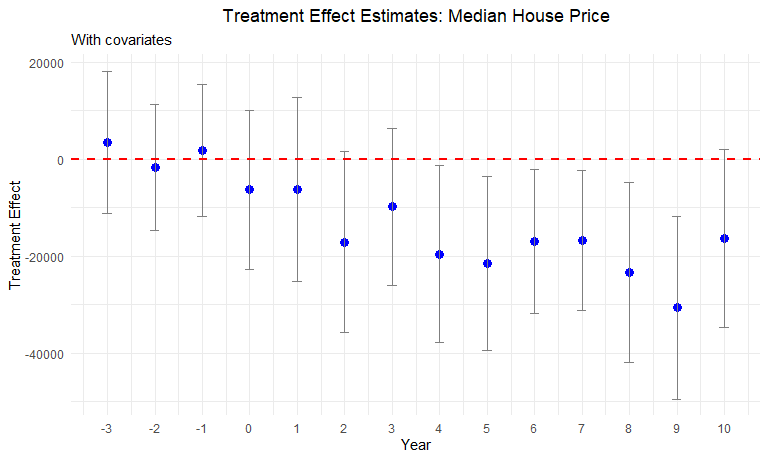
\includegraphics[width=\textwidth,keepaspectratio]{images/tes_gs.png}
%     \caption{Event Study - Median Housing Price}
%     \label{fig:tes_gs_app}
% \end{figure}

% \clearpage


% \subsection{Outcome vs Running variable plots for years after Treatment}

\clearpage

\section{Additional Robustness Tests} \label{sec:appxb}

A fundamental RD assumption is that observations just above and below the threshold are comparable in all aspects except for treatment status. Table \ref{tab:covariate_discontinuity} presents balance tests across key community characteristics at the voting threshold. As shown, demographic and socioeconomic variables—including population size, poverty rates, educational attainment, employment status, and racial composition—exhibit no statistically significant discontinuities at the cutoff. The absence of any discontinuity suggests that our estimated effects on housing prices represent the impact of failing to renew road tax levies rather than pre-existing community differences. This balance verification via a formal RD test, using covariates as the outcome variable, further strengthens our conclusion that the observed housing price effects stem directly from decisions regarding road tax levies, not from underlying differences in community characteristics.

\subsection{Covariate Discontinuity Tables}

\begin{table}[!h]
    \centering
    \caption{Covariate Discontinuity Test Results}
    \label{tab:covariate_discontinuity}
    \begin{tabularx}{\textwidth}{p{4cm}*{3}{X}X}
          \hline
          Variable & Estimate & Std. error & \textit{p-value} & Conf. Interval \\
          \hline
          \renewcommand{\arraystretch}{1.5}
        Population                           & -388      & 1,094   & 0.722  & [-2,532, 1,755] \\
        Poverty Rate                         & 0.017     & 0.014   & 0.234  & [-0.011, 0.045] \\
        Unemployment Rate                 & -0.002    & 0.006   & 0.733  & [-0.013, 0.009] \\
        \% with Kids                         & -0.007    & 0.012   & 0.539  & [-0.030, 0.015] \\
        \% Renters                           & -0.005    & 0.015   & 0.754  & [-0.035, 0.025] \\
        \% White                             & -0.007    & 0.011   & 0.499  & [-0.028, 0.014] \\
        \% Black                             & -0.004    & 0.009   & 0.685  & [-0.021, 0.014] \\
        \% Married                           & -0.013    & 0.015   & 0.374  & [-0.042, 0.016] \\
        \% Separated                         & 0.001     & 0.002   & 0.485  & [-0.002, 0.004] \\
        \% Households with Children under 18 & 0.0001    & 0.007   & 0.981  & [-0.014, 0.014] \\
        \% Less than High School Education   & -0.004    & 0.020   & 0.834  & [-0.043, 0.035] \\
        \% Some College Education            & -0.012    & 0.011   & 0.274  & [-0.034, 0.009] \\
        \hline
    \end{tabularx}
    \begin{tablenotes}
        \small
        \item \textit{Notes:} Estimates indicate the treatment effect of failing to renew a road maintenance tax levy on the value of each covariate considered during our study. 
    \end{tablenotes}
\end{table}

\subsection{Covariate Discontinuity Plots}

% \subsection{Covariate Smoothness Plots}

\begin{figure}[ht]
    \centering
    \begin{minipage}[b]{0.40\textwidth}
        \centering
        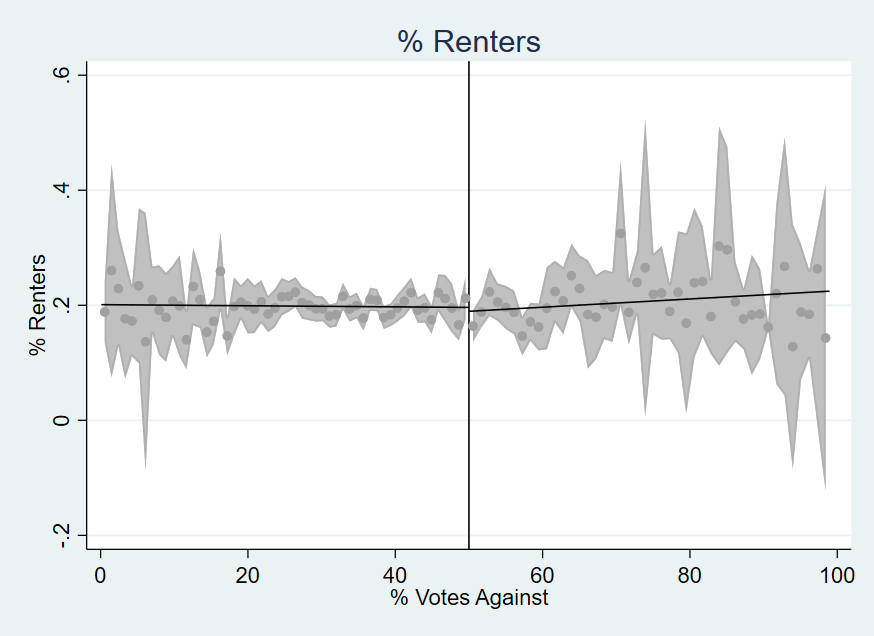
\includegraphics[width=\textwidth,keepaspectratio]{images/cov_smoothness_pctrent.png}
        \caption*{Pct Rent}
        \label{fig:pctrent_sm}
    \end{minipage}
    \hfill
    \begin{minipage}[b]{0.40\textwidth}
        \centering
        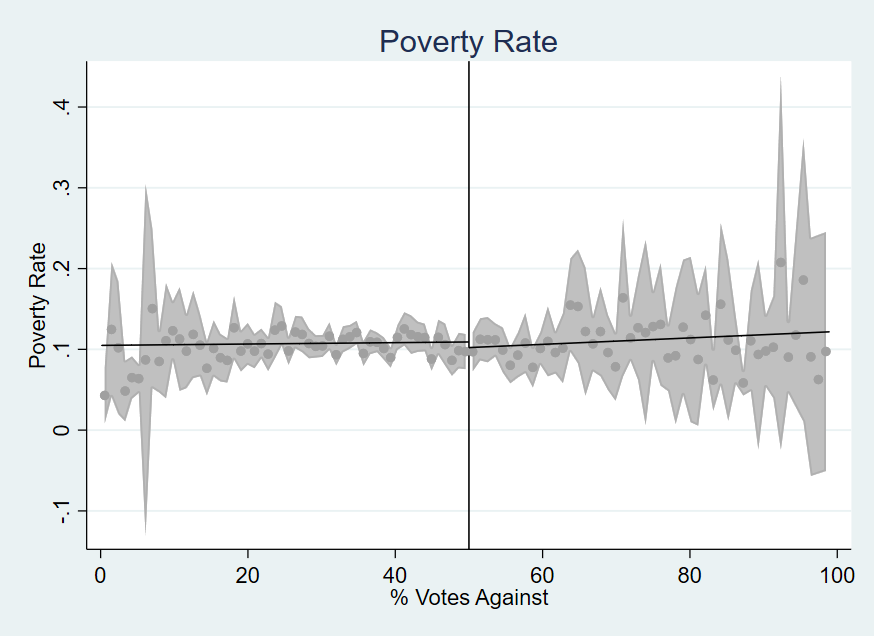
\includegraphics[width=\textwidth,keepaspectratio]{images/cov_smoothness_poverty.png}
        \caption*{Poverty Rate}
        \label{fig:poverty_sm}
    \end{minipage}
    
    % \vspace{1em}
    
    \begin{minipage}[b]{0.40\textwidth}
        \centering
        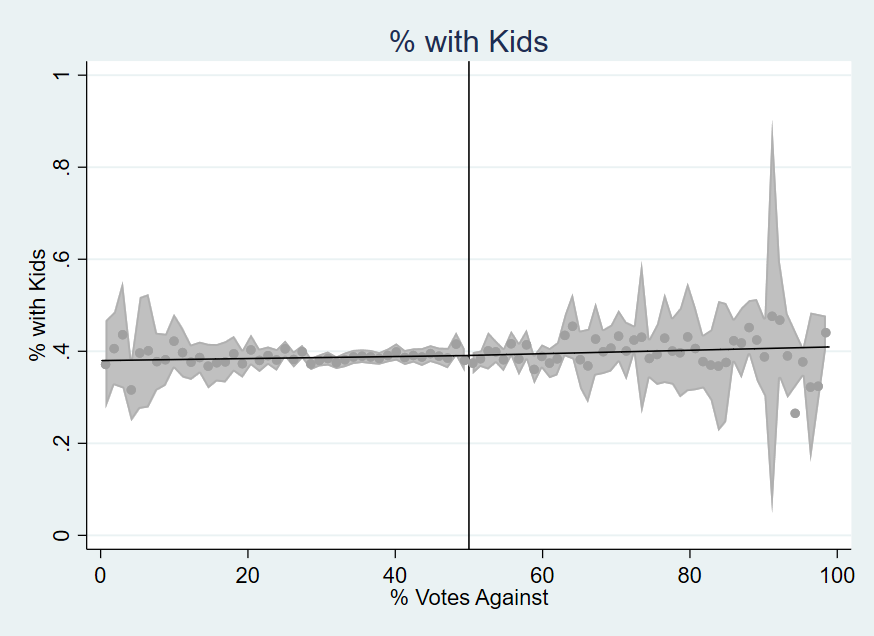
\includegraphics[width=\textwidth,keepaspectratio]{images/cov_smoothness_pctwithkids.png}
        \caption*{Pct With Kids}
        \label{fig:pct_with_kids_sm}
    \end{minipage}
    \hfill
    \begin{minipage}[b]{0.40\textwidth}
        \centering
        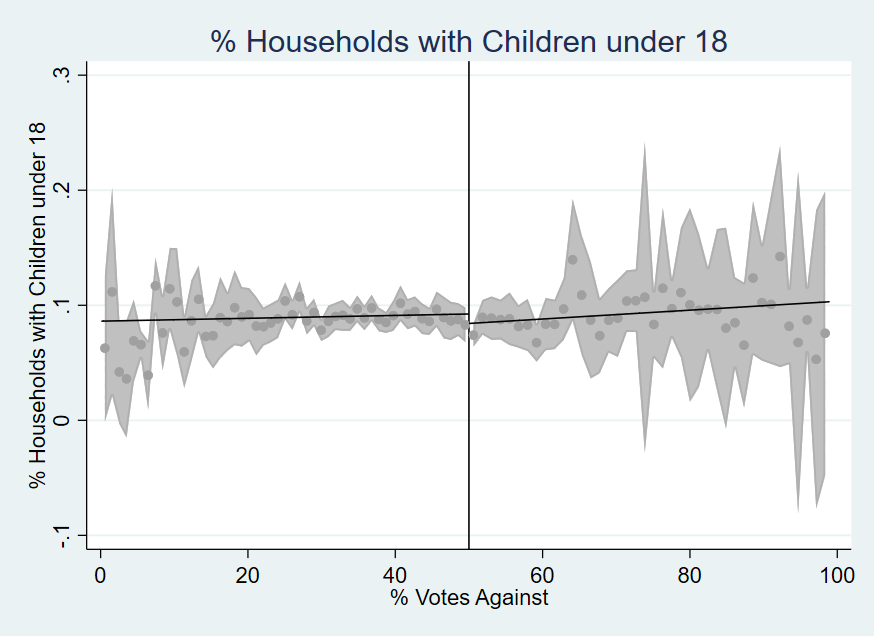
\includegraphics[width=\textwidth,keepaspectratio]{images/cov_smoothness_pctsinparhhld.png}
        \caption*{Pct Single Parent Hhld}
        \label{fig:pctsinparhhld_sm}
    \end{minipage}
    
    % \vspace{1em}
    
    \begin{minipage}[b]{0.40\textwidth}
        \centering
        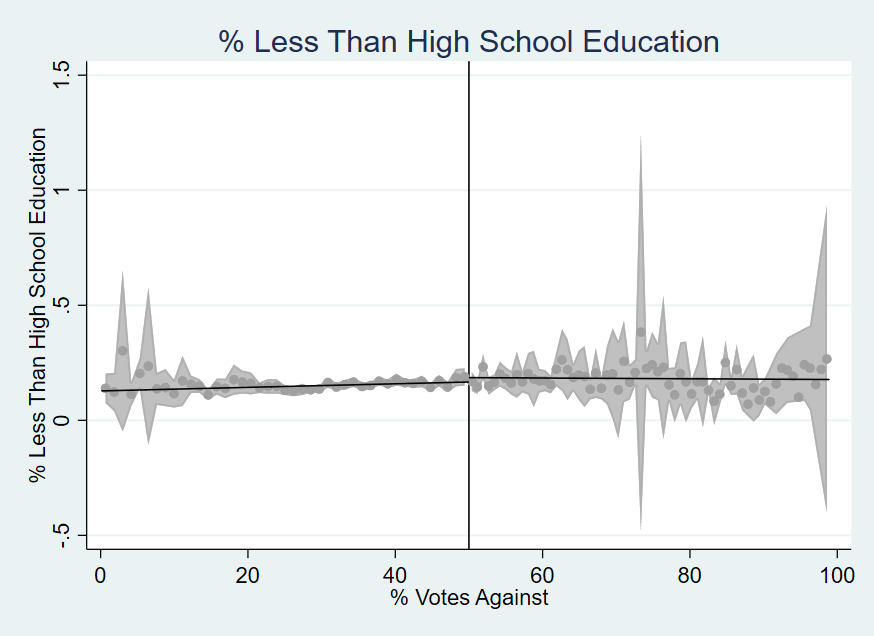
\includegraphics[width=\textwidth,keepaspectratio]{images/cov_smoothness_pctlesshs.png}
        \caption*{Pct Less than HS}
        \label{fig:pctlesshs_sm}
    \end{minipage}
    \hfill
    \begin{minipage}[b]{0.40\textwidth}
        \centering
        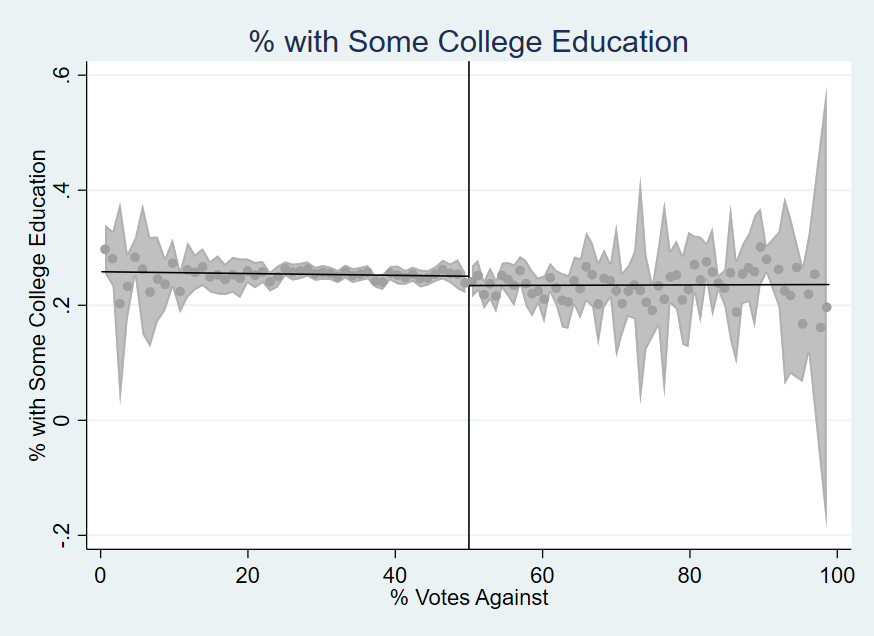
\includegraphics[width=\textwidth,keepaspectratio]{images/cov_smoothness_pctsomecoll.png}
        \caption*{Pct Some College}
        \label{fig:pctsomecoll_sm}
    \end{minipage}
    
    % \vspace{1em}
    
    \begin{minipage}[b]{0.40\textwidth}
        \centering
        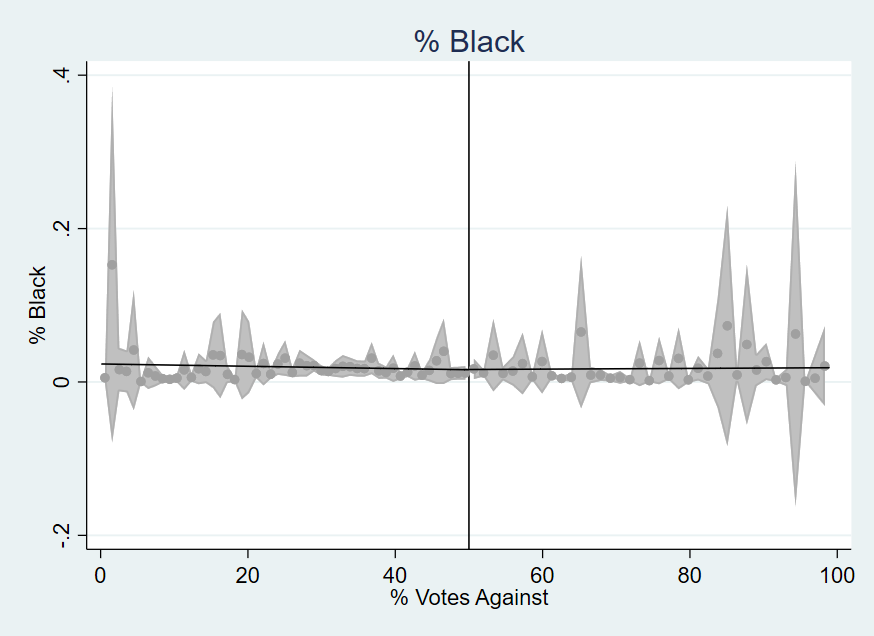
\includegraphics[width=\textwidth,keepaspectratio]{images/cov_smoothness_pctblack.png}
        \caption*{Pct Black}
        \label{fig:black_sm}
    \end{minipage}
    \hfill
    \begin{minipage}[b]{0.40\textwidth}
        \centering
        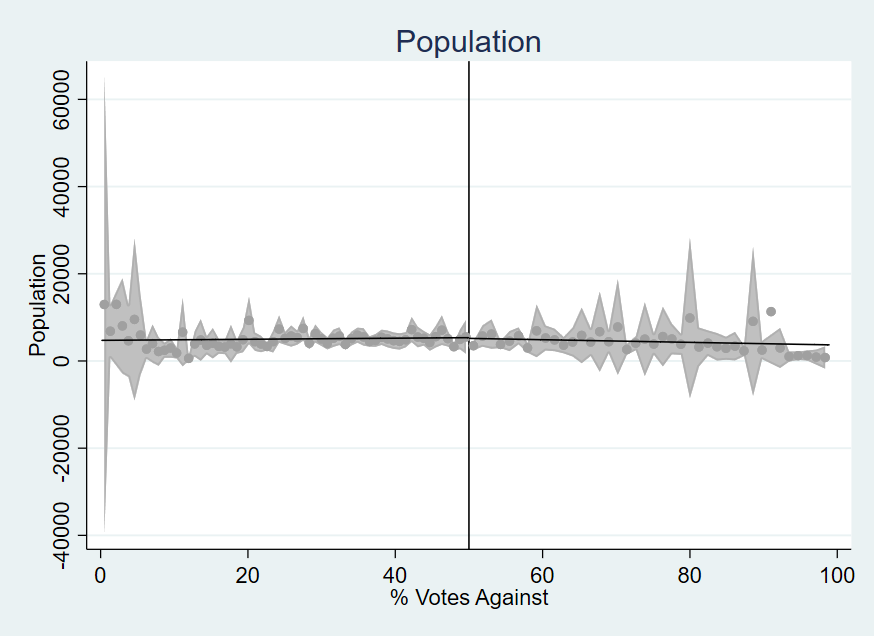
\includegraphics[width=\textwidth,keepaspectratio]{images/cov_smoothness_pop.png}
        \caption*{Population}
        \label{fig:pop_sm}
    \end{minipage}
    
    \caption{Covariate Discontinuity Plots - Part 1}
    \label{fig:rd_cov_smoothness_1}
\end{figure}

\begin{figure}[ht]
    \centering
    \begin{minipage}[b]{0.40\textwidth}
        \centering
        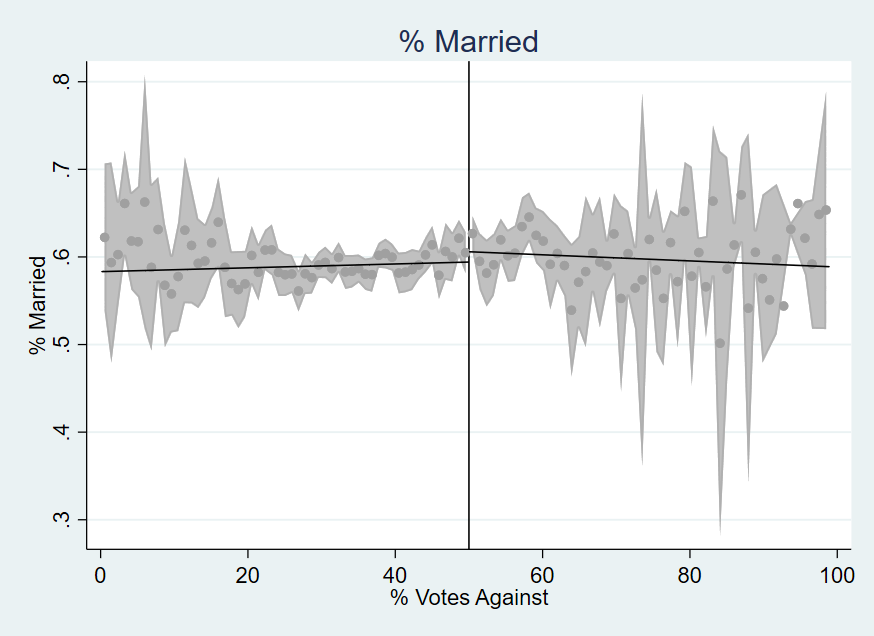
\includegraphics[width=\textwidth,keepaspectratio]{images/cov_smoothness_pctmarried.png}
        \caption*{Pct Married}
        \label{fig:pctmarried_sm}
    \end{minipage}
    \hfill
    \begin{minipage}[b]{0.40\textwidth}
        \centering
        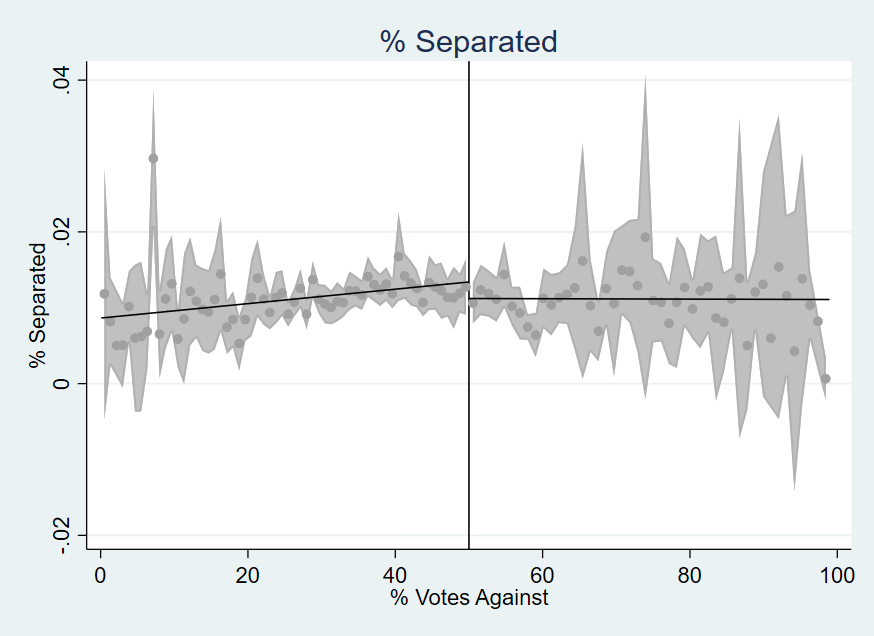
\includegraphics[width=\textwidth,keepaspectratio]{images/cov_smoothness_pctseparated.png}
        \caption*{Pct Separated}
        \label{fig:pctseparated_sm}
    \end{minipage}
    
    \vspace{1em}
    
    \begin{minipage}[b]{0.40\textwidth}
        \centering
        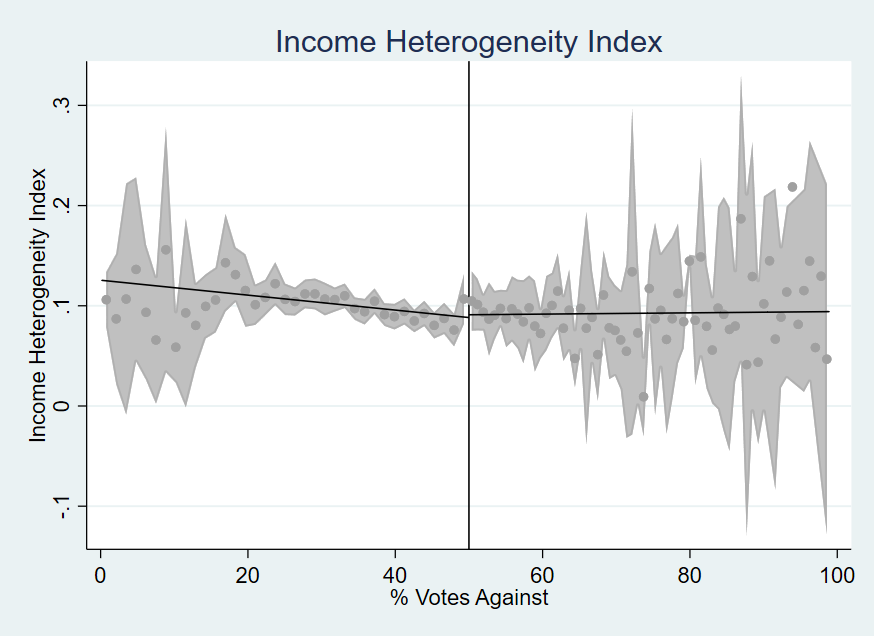
\includegraphics[width=\textwidth,keepaspectratio]{images/cov_smoothness_incherfindahl.png}
        \caption*{Income Herfindahl Index}
        \label{fig:incherfindahl_sm}
    \end{minipage}
    \hfill
    \begin{minipage}[b]{0.40\textwidth}
        \centering
        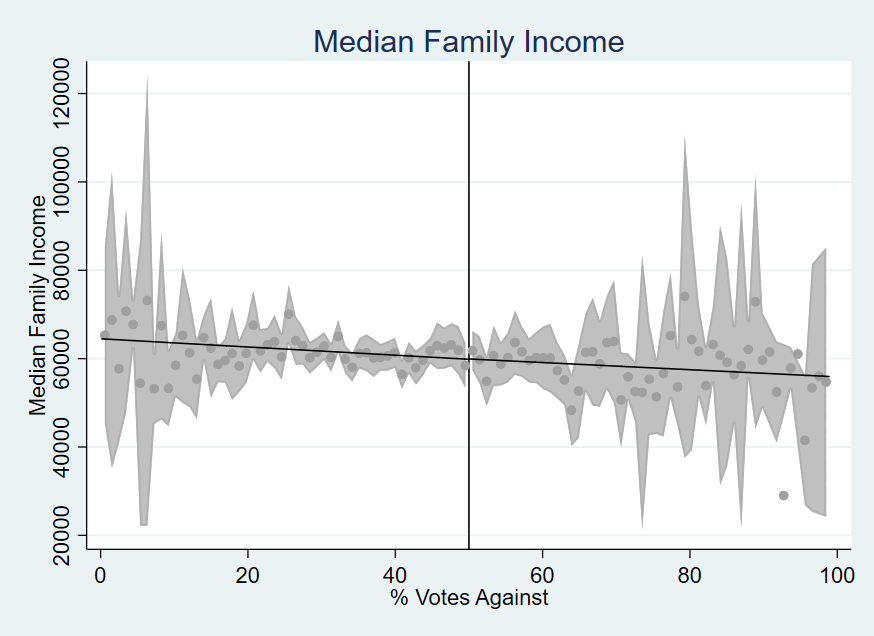
\includegraphics[width=\textwidth,keepaspectratio]{images/cov_smoothness_medfamy.png}
        \caption*{Median Family Income}
        \label{fig:medfamy_sm}
    \end{minipage}
    
    \vspace{1em}
    
    \begin{minipage}[b]{0.40\textwidth}
        \centering
        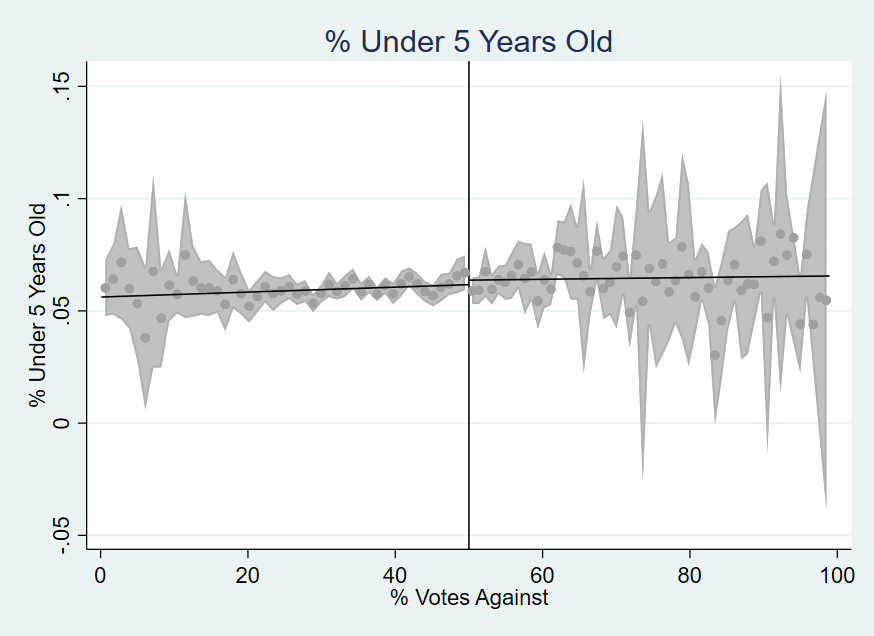
\includegraphics[width=\textwidth,keepaspectratio]{images/cov_smoothness_pctlt5.png}
        \caption*{Pct Less than 5}
        \label{fig:pctlt5_sm}
    \end{minipage}
    \hfill
    \begin{minipage}[b]{0.40\textwidth}
        \centering
        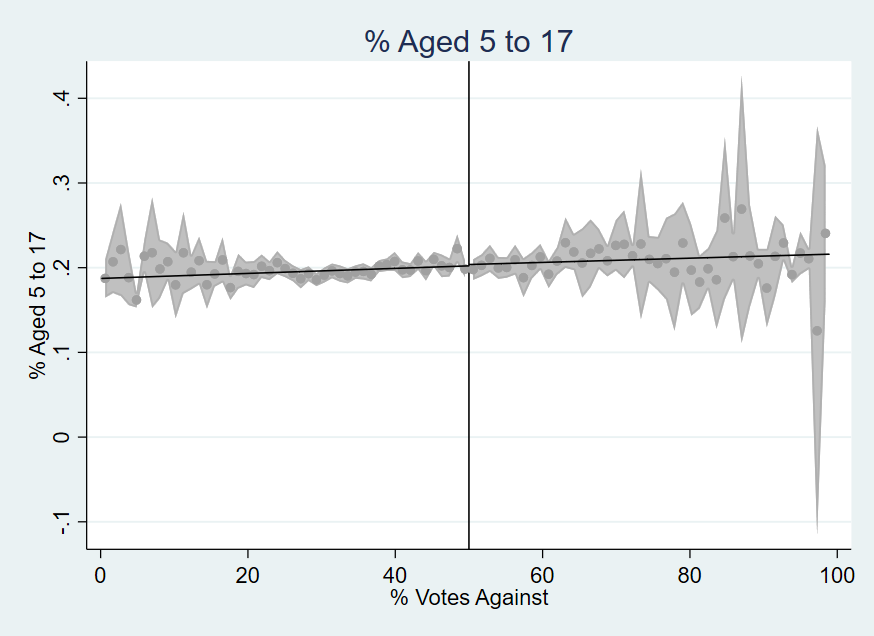
\includegraphics[width=\textwidth,keepaspectratio]{images/cov_smoothness_pct5to17.png}
        \caption*{Pct 5 to 17}
        \label{fig:pct5to17_sm}
    \end{minipage}
    
    \vspace{1em}
    
    \begin{minipage}[b]{0.40\textwidth}
        \centering
        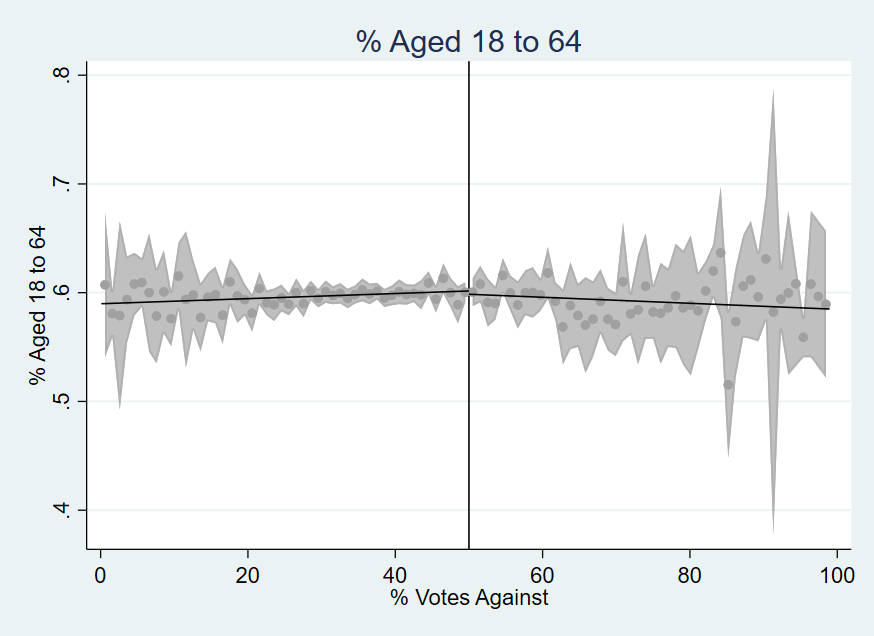
\includegraphics[width=\textwidth,keepaspectratio]{images/cov_smoothness_pct18to64.png}
        \caption*{Pct 18 to 64}
        \label{fig:pct18to64_sm}
    \end{minipage}
    \hfill
    \begin{minipage}[b]{0.40\textwidth}
        \centering
        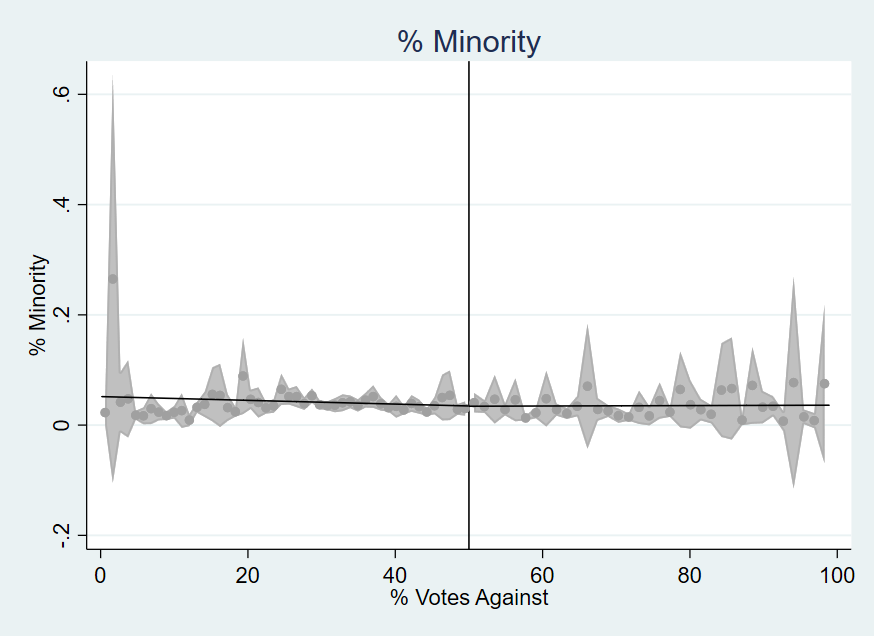
\includegraphics[width=\textwidth,keepaspectratio]{images/cov_smoothness_pctmin.png}
        \caption*{Pct Minority}
        \label{fig:pctmin_sm}
    \end{minipage}
    
    \caption{Covariate Discontinuity Plots - Part 2}
    \label{fig:rd_cov_smoothness_2}
\end{figure}


\clearpage


\section{Additional Information} \label{sec:appxc}

% \subsection{A Case Study of Roads in Waynesville OH: Serial Cutter of Road Maintenance Tax Levies}
% \subsection{More Details on Predicting Road Quality} \label{sec:appxc1} 

% Coming very soon.

\subsection{Road tax levies vs. Other types of levies}

\begin{table}[ht!]
    \centering
    \caption{Correlation of Road Tax Levy Referenda Results with Other Types of Levies}
    \begin{tabular}{lcccccc}
    \toprule
    & Police & Fire & Recreational & School \\
    \midrule
    Estimate & 0.248 & 0.053 & 0.015 & -0.024 \\
    & (0.153) & (0.043) & (0.317) & (0.092) \\
    \bottomrule
    \end{tabular}
    \begin{minipage}{\textwidth}
    \footnotesize
    \textit{Notes:} This table presents coefficients from regressions correlating road tax levy referendum outcomes with outcomes for other types of levies (police, fire, recreational, school). Standard errors are reported in parentheses. All regression control for year and neighborhood fixed effects, as well as neighborhood characteristics. The school levy analysis is conducted at the county level, while all other analyses are at the county subdivisions level. Statistical significance levels are indicated as follows: *** $p<0.01$, ** $p<0.05$, * $p<0.1$.
    \end{minipage}
\end{table}

% \begin{figure}[ht]
%     \centering
%     \begin{minipage}[b]{0.48\textwidth}
%         \centering
%         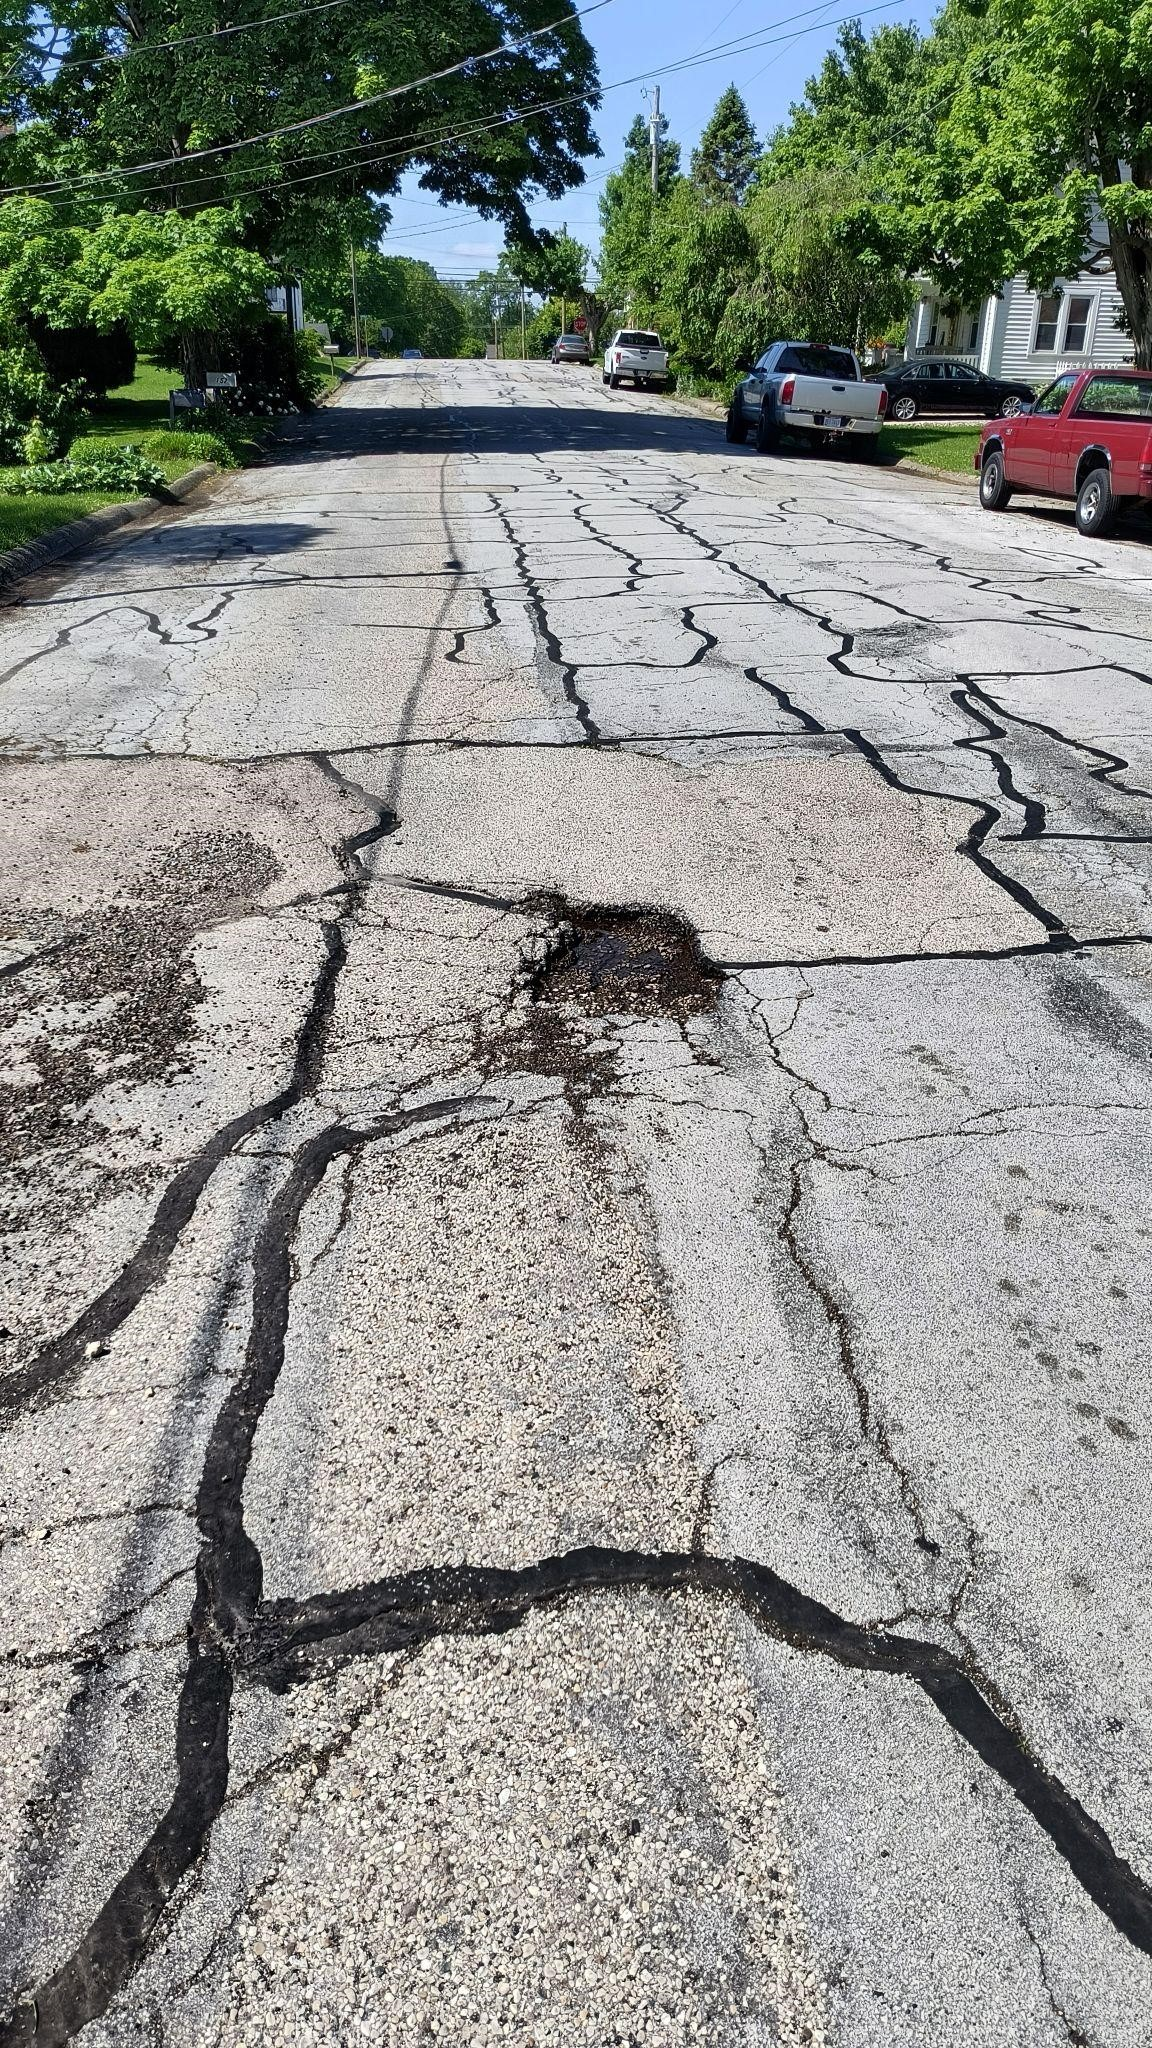
\includegraphics[width=0.75\textwidth,keepaspectratio]{images/waynesville_oh_1.png}
%         \caption*{Waynesville Road Image 1}
%         \label{fig:w_oh_1}
%     \end{minipage}
%     \hfill
%     \begin{minipage}[b]{0.48\textwidth}
%         \centering
%         \includegraphics[width=0.75\textwidth,keepaspectratio]{images/waynesville_oh_2.png}
%         \caption*{Waynesville Road Image 2}
%         \label{fig:w_oh_2}
%     \end{minipage}

%     \vspace{1em}

%     \begin{minipage}[b]{0.48\textwidth}
%         \centering
%         \includegraphics[width=0.75\textwidth,keepaspectratio]{images/waynesville_oh_3.png}
%         \caption*{Waynesville Road Image 3}
%         \label{fig:w_oh_3}
%     \end{minipage}

%     \caption{Roads in Waynesville: Case Study}
%     \label{fig:rd_waynesville}
% \end{figure}

% \section{More Details on Predicting Road Quality} \label{sec:appxd}
